\begin{problem}
  Consider three images $I_1$, $I_2$ and $I_3$ that have been captured
  by a system of three cameras, and suppose the fundamental matrices
  $\bF_{13}$ and $\bF_{23}$ are known. (Notation: the matrix $\bF_{ij}$ satisfies the
  equation $\bx_j^T \bF_{ij} \bx_i = 0$ for any correspondence
  $\bx_i \corr \bx_j$ between images $I_i$ and $I_j$).
  In general, given a point $\bx_1$ in $I_1$ and a corresponding point $\bx_2$ in $I_2$,
  the corresponding point in $\bx_3$ in $I_3$ is uniquely determined
  by the fundamental matrices $\bF_{13}$ and $\bF_{23}$.

  \begin{enumroman}
    \item Write an expression for $\bx_3$ in terms of $\bx_1$, $\bx_2$, $\bF_{13}$ and $\bF_{23}$.
      \begin{answer}
        For a point $x_1 \in I_1$, we can write the epipolar line in $I_3$ as
        \[
          \ell_{31} = \bF_{13} \bx_1.
        \]
        For a point $x_2 \in I_2$, we can write the epipolar line in $I_3$ as
        \[
          \ell_{32} = \bF_{23} \bx_2.
        \]
        The point $\bx_3$ in $I_3$ is the intersection of these two lines, 
        meaning that $\bx_3$ satisfies both the equations
        \[
          \bx_3^T \bF_{13} \bx_1 = 0 \quad \text{and} \quad \bx_3^T \bF_{23} \bx_2 = 0.
        \]
        To find $\bx_3$, use the cross product of the two epipolar lines:
        \[
          \bx_3 = \ell_{31} \times \ell_{32} = \bF_{13}\bx_1 \times \bF_{23} \bx_{2}.
        \]
        Since $\bx_3$ is a point in the image that can be written as
        $\bx_3 = \bmat{x_3 \\ y_3 \\ 1}$, we can write the expression for $\bx_3$ as
        \[
          \bx_3 = \bmat{x_3 \\ y_3 \\ 1} =
          \bF_{13}\bmat{x_{13} \\ y_{13} \\ 1} \times
          \bF_{23} \bmat{x_{23} \\ y_{23} \\ 1}.
        \]
        Thus, we have two unknowns, $x_3$ and $y_3$, and two corresponding equations to solve for them,
        so the point $\bx_3$ is uniquely determined by the fundamental matrices $\bF_{13}$ and $\bF_{23}$.

      \end{answer}

    \newpage
    \item Describe a degenerate configuration of three cameras for which the point $\bx_3$ cannot be
      uniquely determined by this expression.
      \begin{answer}
        A degenerate configuration occurs when the fundamental matrices do not provide
        enough constraints to solve for $\bx_3$. This happens when:
        \begin{enumarabic}
          \item The cameras are collinear, meaning all three cameras are placed
            along the same line. This is an issue because the epipolar lines
            $\ell_{31}$ and $\ell_{32}$ will be parallel, and will never intersect
            (aka intersect at infinity), or intersect at multiple points.
          \item The cameras are coplanar, meaning all three cameras are placed
            in the same exact plane. This is an issue because the epipolar lines
            $\ell_{31}$ and $\ell_{32}$ will be parallel and either never
            intersect (aka intersect at infinity) or intersect at multiple points.
            % image
            \begin{figure}[H]
              \centering
              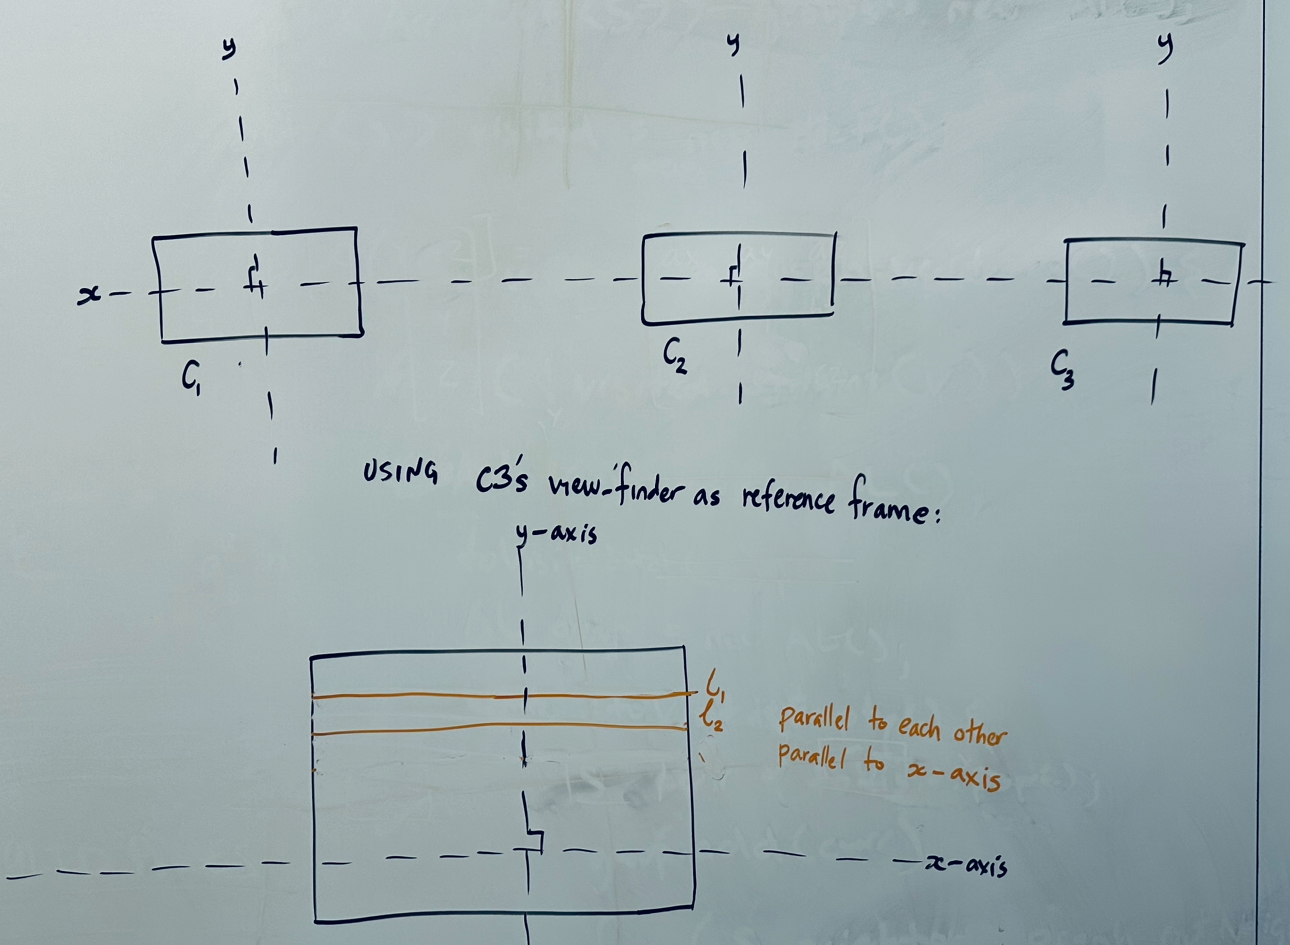
\includegraphics[width=0.7\textwidth]{figures/epipolars.jpg}
              \caption{Epipolar geometry for degenerate configuration.}
              ~\label{fig:2}
            \end{figure}
        \end{enumarabic}
      \end{answer}
  \end{enumroman}

  \emph{
    Hint: Consider the epipolar geometry of the situation. Draw a picture!
  }

\end{problem}
